% ============================================================================
% HR Assistant --- System Architecture Document
% Author: Akram | ICS Compute Internship
% Date: August 2026
% Revised: Full rewrite with breakable tables, landscape diagrams, extended
%          component map, configuration reference, and DB schema details.
% ============================================================================
\documentclass[11pt,a4paper]{article}

% --- Page geometry ---
\usepackage[top=2.5cm, bottom=2.5cm, left=2.5cm, right=2.5cm]{geometry}

% --- Encoding & Language ---
\usepackage[utf8]{inputenc}
\usepackage[T1]{fontenc}
\usepackage[english]{babel}

% --- Fonts ---
\usepackage{lmodern}
\usepackage{microtype}

% --- Colors (matching web app CSS variables) ---
\usepackage[dvipsnames,svgnames,x11names]{xcolor}
\definecolor{Ink}{HTML}{0A0A0A}
\definecolor{InkSoft}{HTML}{1A1A1A}
\definecolor{Muted}{HTML}{5A5852}
\definecolor{Paper}{HTML}{F4F1EA}
\definecolor{PaperDeep}{HTML}{EBE7DD}
\definecolor{PaperLight}{HTML}{FAF8F2}
\definecolor{Red}{HTML}{BC1823}
\definecolor{DeepRed}{HTML}{97121B}
\definecolor{LineBorder}{HTML}{C8C4BC}
\definecolor{SidebarDark}{HTML}{151515}
\definecolor{CodeBg}{HTML}{F8F5EF}
\definecolor{BoxBg}{HTML}{F9F6F0}
\definecolor{SuccessBg}{HTML}{F3F0E8}
\definecolor{WarningBg}{HTML}{FEF5F0}

% --- Graphics and diagrams ---
\usepackage{graphicx}
\usepackage{tikz}
\usetikzlibrary{shapes.geometric, arrows.meta, positioning, fit,
                backgrounds, calc, shadows.blur}

% --- Tables (standard + breakable) ---
\usepackage{booktabs}
\usepackage{tabularx}
\usepackage{ltablex}          % tabularx + longtable = breakable tabularx
\keepXColumns                 % keep X columns in ltablex
\usepackage{longtable}
\usepackage{colortbl}
\usepackage{multirow}
\usepackage{array}

% --- Landscape pages for wide diagrams ---
\usepackage{pdflscape}

% --- Lists ---
\usepackage{enumitem}
\setlist{nosep, leftmargin=1.5em}
\setlist[itemize]{label={\color{Red}\textbullet}}

% --- Code/monospace ---
\usepackage{listings}
\lstset{
  basicstyle=\ttfamily\footnotesize,
  backgroundcolor=\color{CodeBg},
  frame=single,
  rulecolor=\color{LineBorder},
  breaklines=true,
  columns=fullflexible,
  keepspaces=true,
}

% --- Hyperlinks ---
\usepackage[colorlinks=true, linkcolor=Red, urlcolor=DeepRed,
            citecolor=Red, pdfborder={0 0 0}]{hyperref}

% --- Header/Footer ---
\usepackage{fancyhdr}
\pagestyle{fancy}
\fancyhf{}
\fancyhead[L]{\small\color{Muted}\textit{HR Assistant --- System Architecture}}
\fancyhead[R]{\small\color{Muted}\thepage}
\fancyfoot[C]{\small\color{Muted}ICS Compute --- Internship Program 2026}
\renewcommand{\headrulewidth}{0.4pt}
\renewcommand{\footrulewidth}{0.2pt}
\newcommand{\landscapefooter}{%
  \noindent\makebox[\linewidth]{\small\color{Muted}HR Assistant\hfill\thepage}%
}

% --- Section styling ---
\usepackage{titlesec}
\titleformat{\section}
  {\Large\bfseries\color{Red}}
  {\thesection}{1em}{}[\vspace{-0.5em}\textcolor{LineBorder}{\rule{\textwidth}{0.8pt}}]
\titleformat{\subsection}
  {\large\bfseries\color{InkSoft}}
  {\thesubsection}{0.8em}{}
\titleformat{\subsubsection}
  {\normalsize\bfseries\color{Ink}}
  {\thesubsubsection}{0.6em}{}

% --- Custom boxes ---
\usepackage{tcolorbox}
\tcbuselibrary{skins, breakable}

\newtcolorbox{infobox}[1][]{
  enhanced, breakable,
  colback=BoxBg, colframe=Red!70,
  coltitle=white, fonttitle=\bfseries,
  boxrule=0.5pt, arc=3pt,
  left=8pt, right=8pt, top=6pt, bottom=6pt,
  title=#1,
  drop shadow={shadow xshift=0.5mm, shadow yshift=-0.5mm, opacity=0.1},
}
\newtcolorbox{techbox}[1][]{
  enhanced, breakable,
  colback=SuccessBg, colframe=InkSoft!40,
  coltitle=white, fonttitle=\bfseries,
  boxrule=0.5pt, arc=3pt,
  left=8pt, right=8pt, top=6pt, bottom=6pt,
  title=#1,
  drop shadow={shadow xshift=0.5mm, shadow yshift=-0.5mm, opacity=0.1},
}
\newtcolorbox{notebox}{
  enhanced, breakable,
  colback=WarningBg, colframe=Red!40,
  boxrule=0.5pt, arc=3pt,
  left=8pt, right=8pt, top=6pt, bottom=6pt,
}

% --- Paragraph spacing ---
\setlength{\parindent}{0pt}
\setlength{\parskip}{0.6em}

% --- longtable default column separation ---
\setlength{\LTpre}{0.5em}
\setlength{\LTpost}{0.5em}

% --- Document info ---
\title{%
  \vspace{-1cm}
  {\color{Red}\rule{\textwidth}{2pt}}\\[0.8cm]
  {\Huge\bfseries\color{Ink} System Architecture}\\[0.3cm]
  {\LARGE\color{Red} HR Assistant}\\[0.5cm]
  {\color{Red}\rule{\textwidth}{2pt}}
}
\author{}
\date{}

% ============================================================================


\begin{document}
\maketitle
\thispagestyle{empty}
\vfill
\begin{center}
\color{Muted}\small
Dokumentasi teknis arsitektur, alur runtime, data, keamanan,\\
dan deployment aktual HR Assistant.
\end{center}

\newpage
\tableofcontents

\newpage
\section{Konteks Sistem}
\subsection{Tujuan dan Ruang Lingkup}
HR Assistant adalah aplikasi internal berbasis RAG untuk mencari informasi dari SOP, kebijakan HR, dan panduan perusahaan melalui antarmuka percakapan. Jawaban menyertakan citation dan form download ketika tersedia. Admin mengelola dokumen, FAQ, guardrails, activity log, feedback, serta analytics.

\begin{tabularx}{\linewidth}{@{}p{4cm}X@{}}
\toprule \textbf{Area} & \textbf{Kondisi aktual} \\ \midrule
Runtime & Monolith FastAPI pada satu EC2; frontend utama disajikan sebagai static files. \\
Data & PostgreSQL untuk state, analytics, dan metadata cache; ChromaDB lokal untuk document index dan vector semantic cache. \\
AI & 9Router/Kiro untuk chat completion, Nscale untuk embedding, dan Langfuse opsional untuk tracing. \\
Akses & Satu Google sign-in flow. Role admin berasal dari kecocokan email pada \texttt{app.admin\_accounts}. \\
Batas implementasi & HTTPS dan SAML tidak diimplementasikan. Tidak ada HA atau pipeline CI/CD terkelola. \\
\bottomrule
\end{tabularx}

\subsection{Fitur Inti}
\begin{itemize}
  \item Chat RAG dengan conversation history, citations, dan form recommendations.
  \item Context resolution untuk follow-up question dan semantic cache setelah thumbs-up.
  \item Upload dokumen, reindex, FAQ, guardrails, feedback, activity log, dan analytics admin.
  \item Optional reranking dan diagram description jika dependency tersedia.
\end{itemize}

\subsection{Tech Stack}
\begin{tabularx}{\linewidth}{@{}p{3.5cm}X@{}}
\toprule \textbf{Layer} & \textbf{Teknologi} \\ \midrule
Backend & Python 3.12, FastAPI, SQLAlchemy, Alembic, ChromaDB \\
Frontend (User) & Vanilla JS SPA, static HTML/CSS/JS \\
Frontend (Admin) & React 19, TypeScript, Vite, Recharts \\
Database & PostgreSQL 16 \\
Vector Store & ChromaDB (persistent local) \\
AI/LLM & Claude via 9Router/Kiro (OpenAI-compatible API) \\
Embeddings & Nscale (OpenAI-compatible endpoint) \\
Observability & Langfuse (optional tracing) \\
Infrastructure & AWS EC2 (t3.medium), Docker Compose, Nginx \\
\bottomrule
\end{tabularx}

\newpage
\section{Struktur Repository}
\begin{lstlisting}[basicstyle=\ttfamily\scriptsize]
<project-root>/
|-- backend/
|   |-- api/                    # FastAPI routes, auth, storage, models
|   |   |-- main.py             # Application entry point
|   |   |-- core.py             # App factory, middleware, static mounts
|   |   |-- routes_public.py    # Query, conversations, download
|   |   |-- routes_admin.py     # Documents, reindex, FAQ, logs
|   |   |-- routes_auth.py      # Google login flow
|   |   |-- routes_analytics.py # Analytics dashboard routes
|   |   |-- auth.py             # HMAC session + Google verification
|   |   `-- storage.py          # Document and form management
|   |-- researcher_crew/
|   |   `-- src/researcher_crew/
|   |       |-- main.py         # RAG orchestrator
|   |       |-- context_graph.py
|   |       |-- context_schema.py
|   |       `-- tools/custom_tool.py
|   |-- preprocessing/
|   |   |-- ingest.py           # Ingestion entry point
|   |   |-- loader.py           # PDF/DOCX/TXT loader
|   |   |-- chunker.py          # AI chunking + fallback
|   |   |-- diagram_description.py
|   |   |-- embedding.py        # Nscale embeddings
|   |   `-- vectorstore.py      # ChromaDB index
|   |-- analytics/              # Topic and aggregate processing
|   |-- db/
|   |   |-- models.py           # SQLAlchemy ORM
|   |   |-- engine.py           # Synchronous engine/session
|   |   |-- repository.py       # Database operations
|   |   `-- alembic/            # Migration scripts
|   |-- data/                   # Source documents and forms
|   |-- settings.py             # Environment helpers
|   |-- semantic_cache.py
|   `-- observability.py
|-- frontend/
|   |-- web/                    # Main static SPA
|   `-- dashboard/              # React/Vite analytics source
|-- deploy/
|   |-- nginx/hr-agent.conf     # Reverse proxy config
|   `-- update-ec2.sh           # EC2 update script
|-- docs/                       # Architecture and admin guide
|-- docker-compose.yml          # Production services
|-- docker-compose.dev-db.yml   # Local development PostgreSQL
|-- Dockerfile
|-- alembic.ini
|-- requirements.txt
|-- .env.example
|-- run.bat
`-- clean.bat
\end{lstlisting}

\newpage
\section{Ringkasan Arsitektur}
\subsection{Keputusan Utama}
\begin{itemize}
  \item \textbf{Auth:} semua account login dengan Google; admin ditentukan oleh \texttt{app.admin\_accounts}.
  \item \textbf{Session:} token HMAC-SHA256 berlaku 12 jam; role diperiksa kembali dari PostgreSQL.
  \item \textbf{Data:} PostgreSQL menjadi source of truth untuk state dan metadata cache; ChromaDB menyimpan document vectors dan vector index semantic cache.
  \item \textbf{Retrieval:} semantic search dengan optional rerank; jawaban baru di-cache setelah thumbs-up.
  \item \textbf{Runtime:} single-instance deployment dipilih untuk operasional sederhana saat ini.
\end{itemize}

\subsection{Komponen Kode Inti}
\begin{tabularx}{\linewidth}{@{}p{4.8cm}X@{}}
\toprule \textbf{Komponen} & \textbf{Tanggung jawab} \\ \midrule
\texttt{backend/api/*} & FastAPI app, auth, user/admin/analytics routes, storage, FAQ, dan forms. \\
\texttt{backend/}\linebreak\texttt{researcher\_crew/*} & Context graph, retrieval, prompt, dan orchestrator jawaban. \\
\texttt{backend/preprocessing/*} & Loader, visual description, chunking, embedding, dan vector store. \\
\texttt{backend/db/*} & SQLAlchemy synchronous ORM, repository, engine, dan Alembic. \\
\texttt{backend/analytics/*} & Topic classification, canonical interactions, dan daily aggregates. \\
\texttt{frontend/web},\linebreak\texttt{frontend/dashboard} & SPA utama vanilla JS dan dashboard admin React/Vite. \\
\bottomrule
\end{tabularx}



\newpage
\subsection{API Overview}
Semua endpoint berada di bawah FastAPI monolith pada port 8000. Autentikasi menggunakan session token di header.

\begin{tabularx}{\linewidth}{@{}p{2.2cm}p{5.5cm}X@{}}
\toprule \textbf{Method} & \textbf{Endpoint} & \textbf{Deskripsi} \\ \midrule
POST & \texttt{/api/auth/google} & Login via Google ID token, return session. \\
POST & \texttt{/query} & Kirim pertanyaan ke RAG pipeline. \\
GET & \texttt{/api/conversations} & List conversation history user. \\
GET & \texttt{/api/conversations/:id/messages} & Detail messages pada conversation. \\
POST & \texttt{/api/feedback} & Submit feedback (thumbs up/down). \\
GET & \texttt{/api/library} & List dokumen dan form yang dapat diakses. \\
POST & \texttt{/api/admin/documents} & Upload dokumen baru. \\
POST & \texttt{/api/admin/reindex} & Trigger reindex embedding. \\
GET & \texttt{/api/faq} & List FAQ items yang dipublikasikan. \\
GET & \texttt{/api/admin/logs} & Activity log dan session history. \\
GET & \texttt{/api/admin/analytics/*} & Analytics data (overview, charts, topics). \\
GET & \texttt{/health} & Basic health check. \\
\bottomrule
\end{tabularx}

\newpage
\section{Diagram Arsitektur Sistem}
\vspace{0.3cm}
\begin{center}
\resizebox{0.95\linewidth}{!}{%
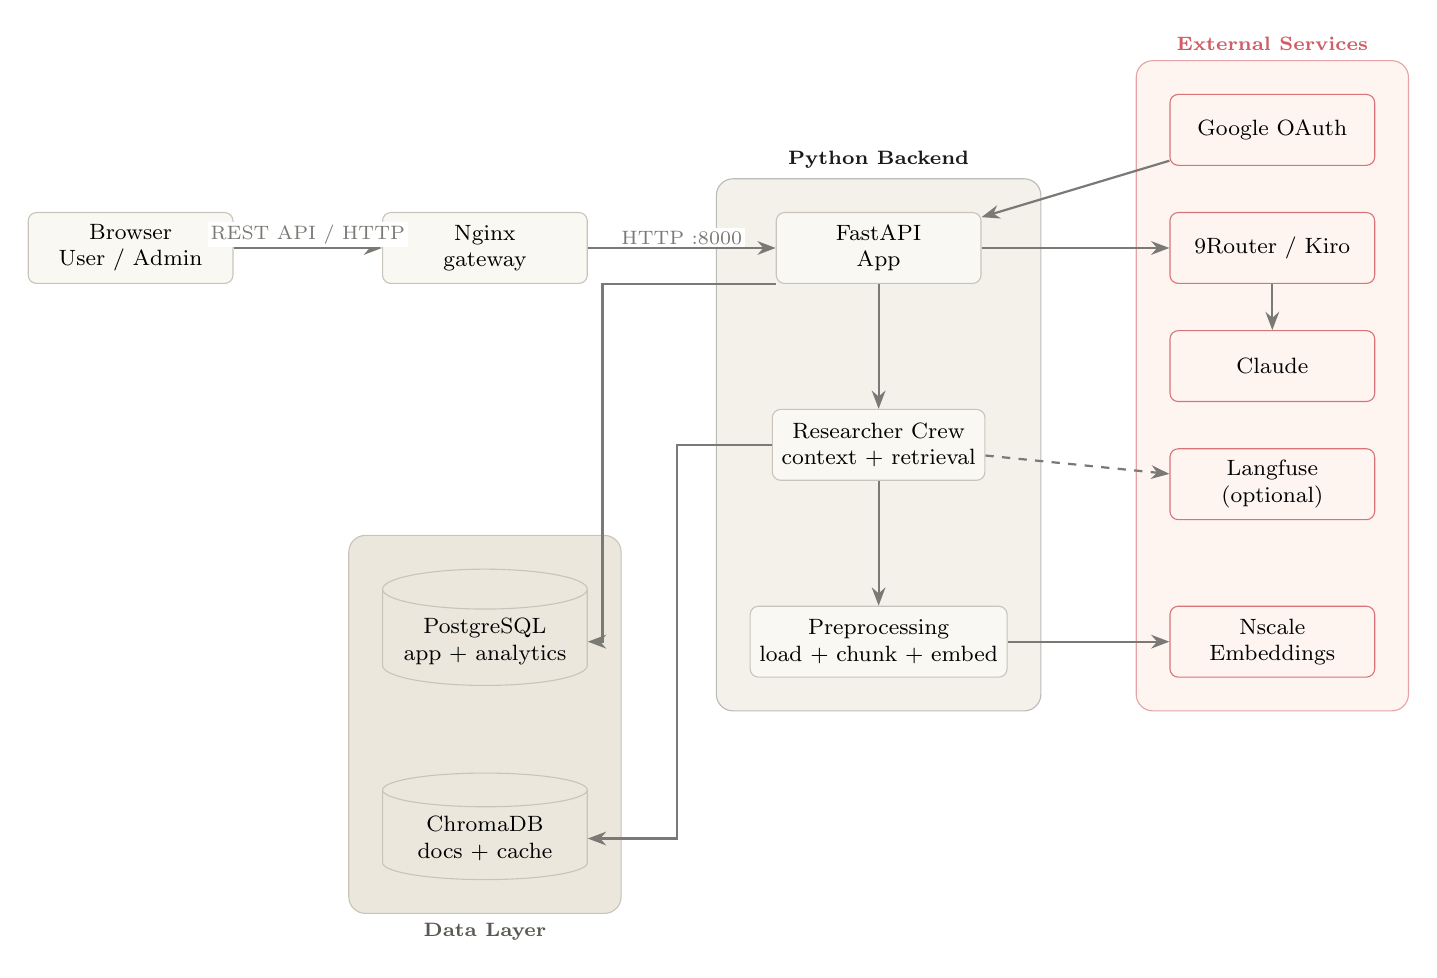
\begin{tikzpicture}[>=Stealth,
  proc/.style={rectangle, rounded corners=3pt, draw=LineBorder, fill=PaperLight,
               minimum width=2.6cm, minimum height=0.9cm, align=center, font=\footnotesize},
  db/.style={cylinder, shape border rotate=90, aspect=.22, draw=LineBorder,
             fill=PaperDeep, minimum width=2.6cm, minimum height=1.0cm,
             align=center, font=\footnotesize},
  ext/.style={rectangle, rounded corners=3pt, draw=Red!60, fill=WarningBg,
              minimum width=2.6cm, minimum height=0.9cm, align=center, font=\footnotesize},
  arr/.style={->, thick, color=Muted!80},
  lbl/.style={font=\scriptsize, fill=white, inner sep=1pt}
]

%% ---- Frontend layer (top-left) ----
\begin{scope}
  \node[proc] (browser) at (0, 0) {Browser\\User / Admin};
\end{scope}

%% ---- Gateway ----
\node[proc] (nginx) at (4.5, 0) {Nginx\\gateway};

%% ---- Backend layer box ----
\node[proc] (fastapi) at (9.5, 0) {FastAPI\\App};
\node[proc] (rag)     at (9.5,-2.5) {Researcher Crew\\context + retrieval};
\node[proc] (ingest)  at (9.5,-5.0) {Preprocessing\\load + chunk + embed};

%% ---- Data layer ----
\node[db]   (pg)      at (4.5,-5.0) {PostgreSQL\\app + analytics};
\node[db]   (chroma)  at (4.5,-7.5) {ChromaDB\\docs + cache};

%% ---- External services ----
\node[ext] (google)  at (14.5,  1.5) {Google OAuth};
\node[ext] (router)  at (14.5,  0.0) {9Router / Kiro};
\node[ext] (claude)  at (14.5, -1.5) {Claude};
\node[ext] (nscale)  at (14.5, -5.0) {Nscale\\Embeddings};
\node[ext] (langfuse) at (14.5, -3.0) {Langfuse\\(optional)};

%% Background: Backend box
\begin{scope}[on background layer]
  \node[draw=InkSoft!30, fill=Paper, rounded corners=6pt,
        inner sep=12pt, fit=(fastapi)(rag)(ingest), label={[font=\scriptsize\bfseries, color=InkSoft]above:Python Backend}] {};
\end{scope}

%% Background: Data layer box
\begin{scope}[on background layer]
  \node[draw=LineBorder, fill=PaperDeep, rounded corners=6pt,
        inner sep=12pt, fit=(pg)(chroma), label={[font=\scriptsize\bfseries, color=Muted]below:Data Layer}] {};
\end{scope}

%% Background: External services box
\begin{scope}[on background layer]
  \node[draw=Red!40, fill=WarningBg, rounded corners=6pt,
        inner sep=12pt, fit=(google)(router)(claude)(nscale)(langfuse),
        label={[font=\scriptsize\bfseries, color=Red!70]above:External Services}] {};
\end{scope}

%% ---- Arrows ----
\draw[arr] (browser) -- node[lbl, above]{REST API / HTTP} (nginx);
\draw[arr] (nginx)   -- node[lbl, above]{HTTP :8000} (fastapi);
\draw[arr] (fastapi) -- (rag);
\draw[arr] (rag) -- (ingest);
\draw[arr] (fastapi) -- (router);
% Route FastAPI->PG from the south-west corner (below the Nginx->FastAPI row)
% on an outer channel so it never crosses the RAG->ChromaDB channel below.
\draw[arr] (fastapi.south west) -- ++(-2.2,0) |- (pg.east);
% Route RAG->ChromaDB on an inner channel, closer to the backend column.
\draw[arr] (rag.west) -- ++(-1.2,0) |- (chroma.east);
\draw[arr] (ingest)  -- (nscale);
\draw[arr] (router)  -- (claude);
\draw[arr] (google)  -- (fastapi);
\draw[arr, dashed] (rag) -- (langfuse);

\end{tikzpicture}%
}
\end{center}
\begin{center}\small\color{Muted}Dependency runtime utama; external services ditandai outline merah.\end{center}

\newpage
\section{Data dan Konfigurasi}
\subsection{Model Data Inti}
\begin{tabularx}{\linewidth}{@{}p{5.1cm}X@{}}
\toprule \textbf{Tabel} & \textbf{Peran} \\ \midrule
\texttt{app.users}, \texttt{app.admin\_accounts} & Identitas Google dan allowlist role admin tanpa password. \\
\texttt{app.conversations}, \texttt{app.conversation\_messages} & Riwayat chat dan metadata jawaban, citation, serta form. \\
\texttt{app.faq\_items} & FAQ berbasis knowledge base beserta citation metadata. \\
\texttt{app.activity\_logs}, \texttt{app.semantic\_cache\_entries} & Log/feedback produk dan metadata semantic cache. \\
\texttt{analytics.canonical\_}\linebreak\texttt{interactions} & Interaksi ternormalisasi untuk analytics. \\
\texttt{analytics.daily\_topic\_}\linebreak\texttt{aggregates} & Rollup harian topic, user, feedback, dan fallback/error. \\
\texttt{app.app\_state\_meta} & Session signing, guardrails, dan metadata state. \\
\bottomrule
\end{tabularx}

\subsection{Konfigurasi Wajib}
\begin{tabularx}{\linewidth}{@{}p{5.1cm}X@{}}
\toprule \textbf{Variable / group} & \textbf{Fungsi} \\ \midrule
\texttt{DATABASE\_URL} & PostgreSQL connection string. \\
\texttt{MODEL}, \texttt{CHAT\_BASE\_URL} & Model chat dan endpoint 9Router/OpenAI-compatible. \\
\texttt{NSCALE\_SERVICE\_TOKEN}, \texttt{EMBED\_MODEL} & Credential dan model embedding. \\
\texttt{GOOGLE\_CLIENT\_ID} & Verifikasi Google login dan rendering sign-in. \\
\texttt{DATA\_DIR}, \texttt{CHROMA\_DIR}, \texttt{SEMANTIC\_CACHE\_DIR} & Source documents dan persistent vector stores. \\
\texttt{LANGFUSE\_*} & Tracing opsional; switch default aktif dan IO mode masked. \\
\bottomrule
\end{tabularx}

\newpage
\begin{landscape}
\thispagestyle{empty}
\section{Alur Chat End-to-End}
\vspace{0.3cm}
\begin{center}
\resizebox{0.97\linewidth}{!}{%
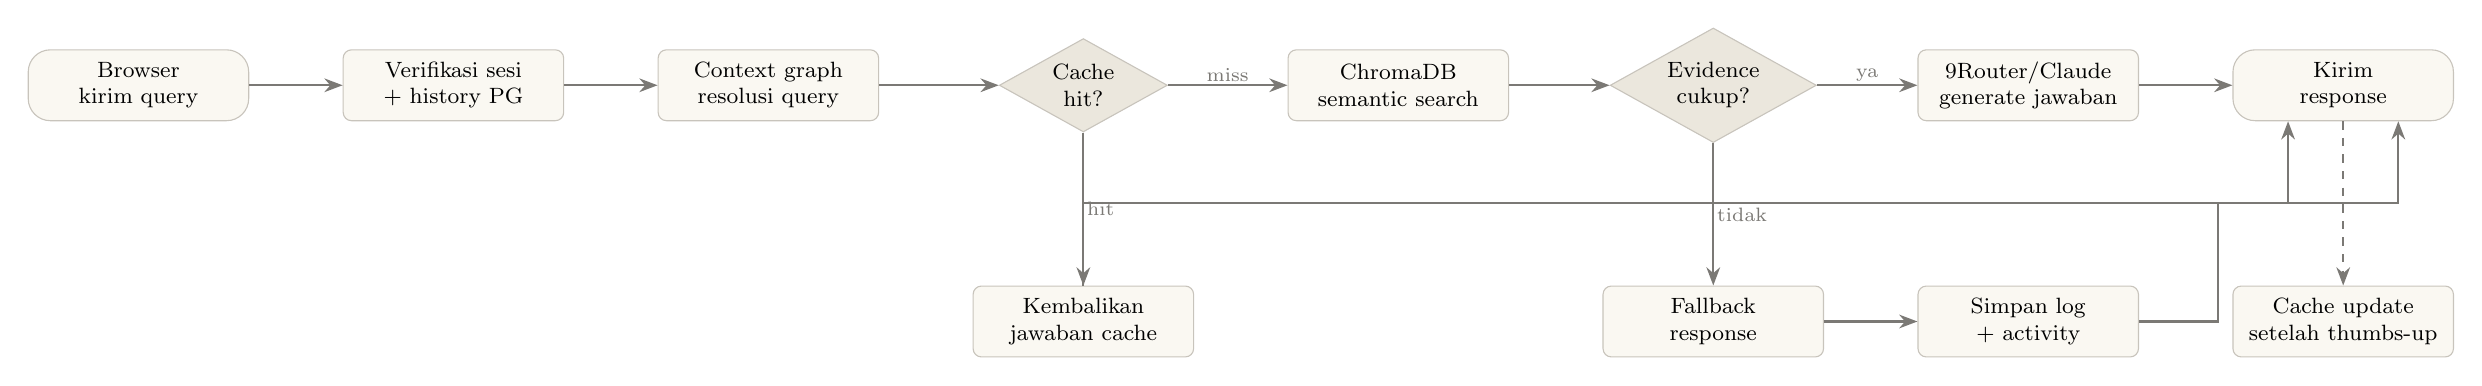
\begin{tikzpicture}[>=Stealth,
  proc/.style={rectangle, rounded corners=3pt, draw=LineBorder, fill=PaperLight,
               minimum width=2.8cm, minimum height=0.9cm, align=center, font=\footnotesize},
  dec/.style={diamond, draw=LineBorder, fill=PaperDeep, aspect=1.8,
              align=center, font=\footnotesize, inner sep=2pt},
  term/.style={rectangle, rounded corners=8pt, draw=LineBorder, fill=PaperLight,
               minimum width=2.8cm, minimum height=0.9cm, align=center, font=\footnotesize},
  arr/.style={->, thick, color=Muted!80},
  lbl/.style={font=\scriptsize, fill=white, inner sep=1pt}
]

%% ---- Row 1: main happy path (left to right, y=0) ----
\node[term]  (start)   at ( 0.0,  0) {Browser\\kirim query};
\node[proc]  (verify)  at ( 4.0,  0) {Verifikasi sesi\\+ history PG};
\node[proc]  (context) at ( 8.0,  0) {Context graph\\resolusi query};
\node[dec]   (cachehit) at (12.0,  0) {Cache\\hit?};
\node[proc]  (search)  at (16.0,  0) {ChromaDB\\semantic search};
\node[dec]   (enough)  at (20.0,  0) {Evidence\\cukup?};
\node[proc]  (llm)     at (24.0,  0) {9Router/Claude\\generate jawaban};
\node[term]  (send)    at (28.0,  0) {Kirim\\response};

%% ---- Row 2: branch paths (y = -3) ----
\node[proc]  (cached)  at (12.0, -3) {Kembalikan\\jawaban cache};
\node[proc]  (fallback) at (20.0, -3) {Fallback\\response};
\node[proc]  (save)    at (24.0, -3) {Simpan log\\+ activity};

%% ---- Main path arrows ----
\draw[arr] (start)   -- (verify);
\draw[arr] (verify)  -- (context);
\draw[arr] (context) -- (cachehit);
\draw[arr] (cachehit) -- node[lbl, above]{miss} (search);
\draw[arr] (search)  -- (enough);
\draw[arr] (enough)  -- node[lbl, above]{ya} (llm);
\draw[arr] (llm)     -- (send);

%% ---- Cache hit branch ----
\draw[arr] (cachehit) -- node[lbl, right]{hit} (cached);
% Return lane sits between row 1 and row 2 so it never overlaps either row;
% enters "send" slightly left of centre to stay clear of the save-branch arrow.
\draw[arr] (cached.north) -- ++(0,1.05) -| ($(send.south)+(-0.7,0)$);

%% ---- Not enough evidence branch ----
\draw[arr] (enough)  -- node[lbl, right]{tidak} (fallback);
\draw[arr] (fallback) -- (save);
%% ---- Cache note below send ----
\node[proc, minimum width=2.8cm] (cachewrite) at (28.0, -3) {Cache update\\setelah thumbs-up};
% Return lane routed around the cache-write node below "send" (avoids the
% coordinate (28,-3), which is where cachewrite sits), entering slightly right.
\draw[arr] (save.east) -- ++(1.0,0) -- ++(0,1.5) -| ($(send.south)+(0.7,0)$);
\draw[arr, dashed] (send) -- (cachewrite);

\end{tikzpicture}%
}
\end{center}
\begin{center}\small\color{Muted}Alur utama (atas) dan jalur alternatif (bawah); cache hanya diperbarui setelah feedback positif.\end{center}
\vfill
\landscapefooter
\end{landscape}

\newpage
\begin{landscape}
\thispagestyle{empty}
\section{Alur Ingestion Dokumen}
\vspace{0.3cm}
\begin{center}
\resizebox{0.97\linewidth}{!}{%
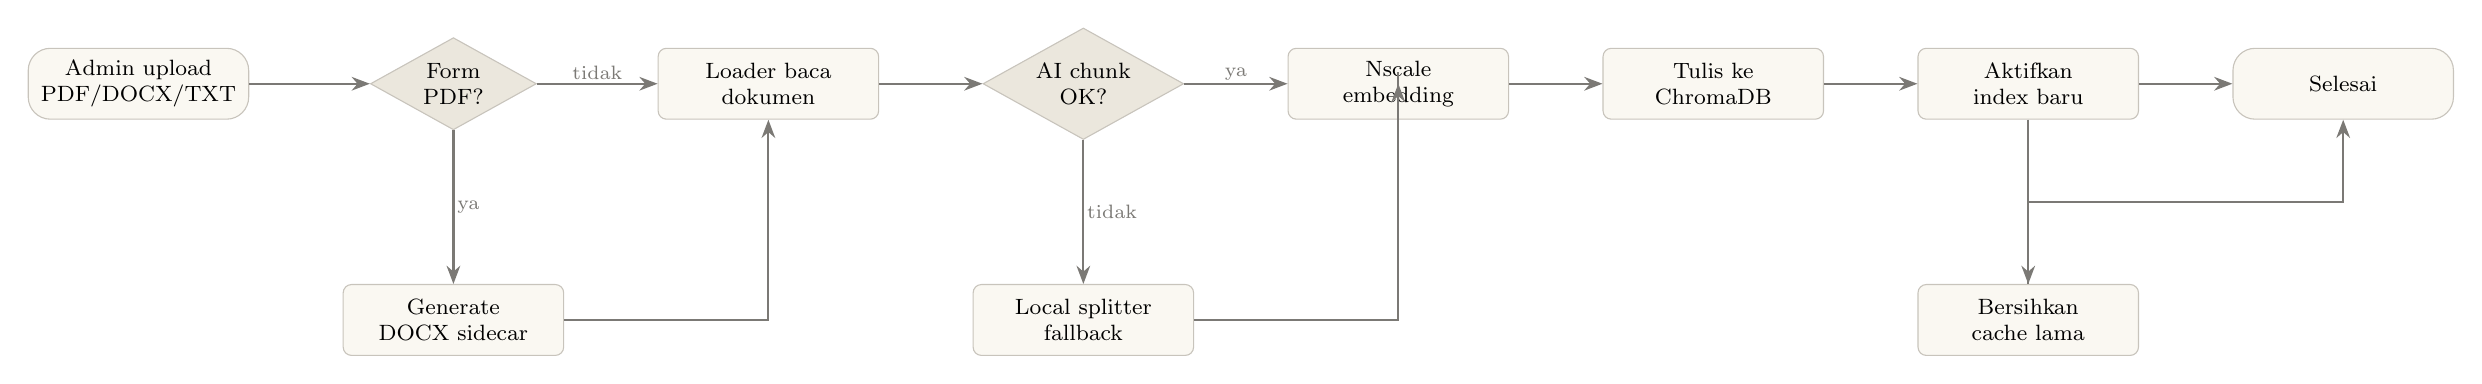
\begin{tikzpicture}[>=Stealth,
  proc/.style={rectangle, rounded corners=3pt, draw=LineBorder, fill=PaperLight,
               minimum width=2.8cm, minimum height=0.9cm, align=center, font=\footnotesize},
  dec/.style={diamond, draw=LineBorder, fill=PaperDeep, aspect=1.8,
              align=center, font=\footnotesize, inner sep=2pt},
  term/.style={rectangle, rounded corners=8pt, draw=LineBorder, fill=PaperLight,
               minimum width=2.8cm, minimum height=0.9cm, align=center, font=\footnotesize},
  arr/.style={->, thick, color=Muted!80},
  lbl/.style={font=\scriptsize, fill=white, inner sep=1pt}
]

%% ---- Row 1: main path (left to right, y=0) ----
\node[term]  (upload)   at ( 0.0,  0) {Admin upload\\PDF/DOCX/TXT};
\node[dec]   (formpdf)  at ( 4.0,  0) {Form\\PDF?};
\node[proc]  (loader)   at ( 8.0,  0) {Loader baca\\dokumen};
\node[dec]   (aichunk)  at (12.0,  0) {AI chunk\\OK?};
\node[proc]  (embed)    at (16.0,  0) {Nscale\\embedding};
\node[proc]  (store)    at (20.0,  0) {Tulis ke\\ChromaDB};
\node[proc]  (activate) at (24.0,  0) {Aktifkan\\index baru};
\node[term]  (done)     at (28.0,  0) {Selesai};

%% ---- Row 2: branch paths (y = -3) ----
\node[proc]  (sidecar)  at ( 4.0, -3) {Generate\\DOCX sidecar};
\node[proc]  (fallback) at (12.0, -3) {Local splitter\\fallback};
\node[proc]  (clearcache) at (24.0, -3) {Bersihkan\\cache lama};

%% ---- Main path arrows ----
\draw[arr] (upload)  -- (formpdf);
\draw[arr] (formpdf) -- node[lbl, above]{tidak} (loader);
\draw[arr] (loader)  -- (aichunk);
\draw[arr] (aichunk) -- node[lbl, above]{ya} (embed);
\draw[arr] (embed)   -- (store);
\draw[arr] (store)   -- (activate);
\draw[arr] (activate) -- (done);

%% ---- Form PDF branch ----
\draw[arr] (formpdf) -- node[lbl, right]{ya} (sidecar);
\draw[arr] (sidecar) -- ++(4.0, 0) -- (loader);

%% ---- AI chunk fail branch ----
\draw[arr] (aichunk) -- node[lbl, right]{tidak} (fallback);
\draw[arr] (fallback) -- ++(4.0, 0) -- ++(0, 3.0) -- (embed);

%% ---- Clear old cache (linked from activate) ----
\draw[arr] (activate) -- ++(0, -1.5) -- (clearcache);
\draw[arr] (clearcache) -- ++(0, 1.5) -| (done);

\end{tikzpicture}%
}
\end{center}
\begin{center}\small\color{Muted}Alur ingestion utama (atas); sidecar PDF dan fallback chunking ditampilkan di baris bawah.\end{center}
\vfill
\landscapefooter
\end{landscape}

\newpage
\section{Keamanan dan Otorisasi}
\begin{tabularx}{\linewidth}{@{}p{4.4cm}X@{}}
\toprule \textbf{Kontrol} & \textbf{Implementasi aktual} \\ \midrule
Authentication & Google ID token untuk semua user/admin; hosted domain divalidasi. \\
Admin role & Email pada \texttt{app.admin\_accounts} berarti admin; email lain berarti user. \\
Session & HMAC-SHA256, expiry 12 jam, secret acak di PostgreSQL; logout menghapus sesi lokal dan menonaktifkan Google auto-select. \\
Authorization & FastAPI dependencies membedakan user/admin dan memeriksa row user live. \\
File handling & Validasi extension, ukuran, path traversal, document kind, dan replacement path. \\
Privacy & Analytics memakai pseudonymous user ID; Langfuse masked mode meredaksi pola sensitif. \\
Gap & Belum ada rate limiting, server-side token revocation list, dependency scan, atau TLS termination. \\
\bottomrule
\end{tabularx}



\newpage
\section{Deployment Aktual EC2}

\begin{center}
\resizebox{0.95\linewidth}{!}{%
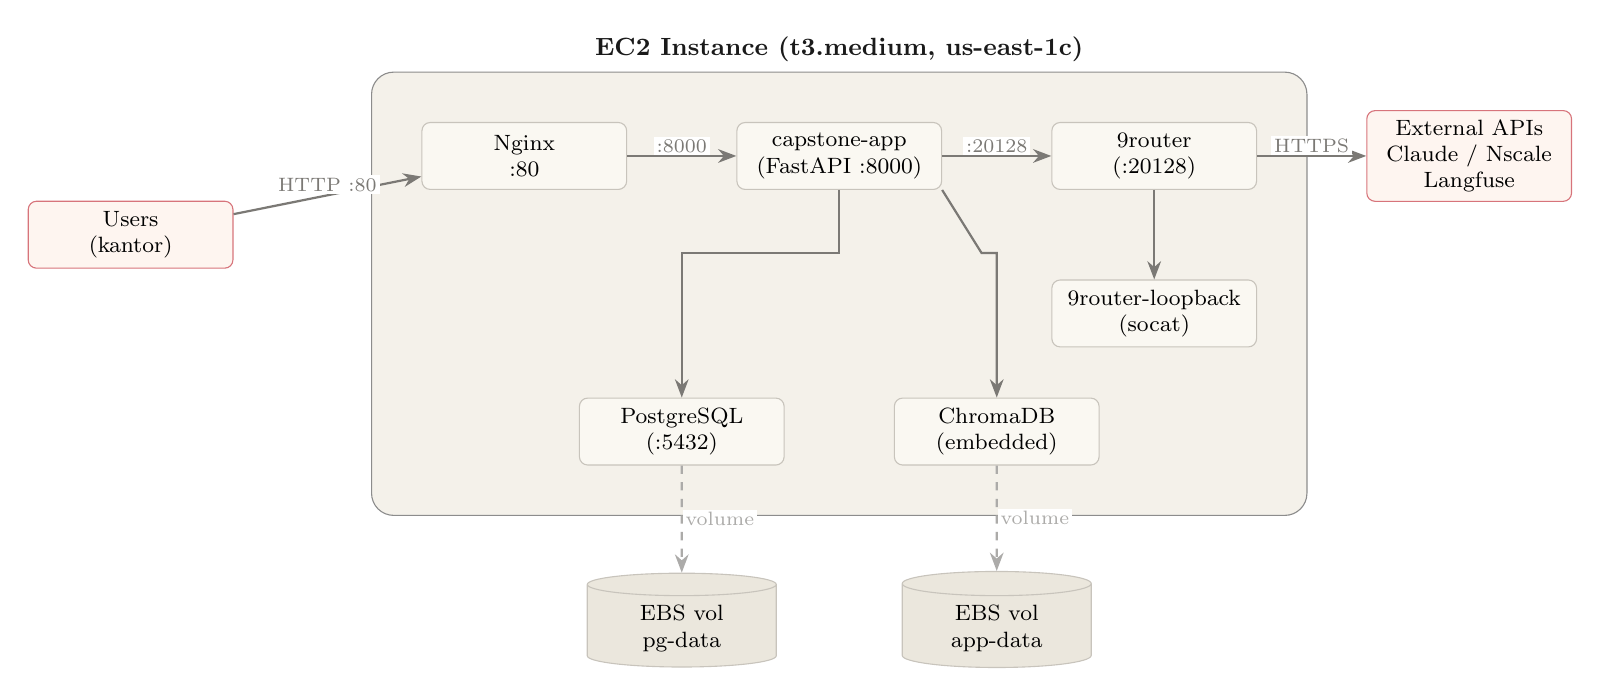
\begin{tikzpicture}[>=Stealth,
  proc/.style={rectangle, rounded corners=3pt, draw=LineBorder, fill=PaperLight,
               minimum width=2.6cm, minimum height=0.85cm, align=center, font=\footnotesize},
  ext/.style={rectangle, rounded corners=3pt, draw=Red!60, fill=WarningBg,
              minimum width=2.6cm, minimum height=0.85cm, align=center, font=\footnotesize},
  store/.style={cylinder, shape border rotate=90, aspect=.22, draw=LineBorder,
                fill=PaperDeep, minimum width=2.4cm, minimum height=0.9cm,
                align=center, font=\footnotesize},
  arr/.style={->, thick, color=Muted!80},
  darr/.style={->, thick, color=Muted!50, dashed},
  lbl/.style={font=\scriptsize, fill=white, inner sep=1pt}
]

%% ---- Outside EC2: Users (left) ----
\node[ext] (users) at (-3.5, 1.0) {Users\\(kantor)};

%% ---- Inside EC2: containers ----
\node[proc] (nginx)      at ( 1.5,  2.0) {Nginx\\:80};
\node[proc] (app)        at ( 5.5,  2.0) {capstone-app\\(FastAPI :8000)};
\node[proc] (router)     at ( 9.5,  2.0) {9router\\(:20128)};
\node[proc] (loopback)   at ( 9.5,  0.0) {9router-loopback\\(socat)};
\node[proc] (pg)         at ( 3.5, -1.5) {PostgreSQL\\(:5432)};
\node[proc] (chroma)     at ( 7.5, -1.5) {ChromaDB\\(embedded)};

%% ---- Outside EC2: External APIs (right) ----
\node[ext] (extapi) at (13.5, 2.0) {External APIs\\Claude / Nscale\\Langfuse};

%% ---- Below EC2: EBS storage ----
% Positioned so each volume sits directly under its owning service,
% keeping the connector lines below straight instead of crossing.
\node[store] (ebs1) at ( 3.5, -4.0) {EBS vol\\pg-data};
\node[store] (ebs2) at ( 7.5, -4.0) {EBS vol\\app-data};

%% ---- EC2 boundary box ----
\begin{scope}[on background layer]
  \node[draw=InkSoft!50, fill=Paper, rounded corners=8pt, inner sep=18pt,
        fit=(nginx)(app)(router)(loopback)(pg)(chroma),
        label={[font=\small\bfseries, color=InkSoft]above:EC2 Instance (t3.medium, us-east-1c)}] (ec2box) {};
\end{scope}

%% ---- Traffic flow arrows ----
\draw[arr] (users)   -- node[lbl, above]{HTTP :80} (nginx);
\draw[arr] (nginx)   -- node[lbl, above]{:8000} (app);
\draw[arr] (app)     -- node[lbl, above]{:20128} (router);
\draw[arr] (router)  -- node[lbl, above]{HTTPS} (extapi);
\draw[arr] (router)  -- (loopback);
% Route app->pg going down then left to avoid crossing any node
\draw[arr] (app.south) -- ++(0,-0.8) -| (pg.north);
% Route app->chroma going down-right orthogonally
\draw[arr] (app.south east) -- ++(0.5,-0.8) -| (chroma.north);

%% ---- EBS dashed connections ----
\draw[darr] (pg)     -- node[lbl, right]{volume} (ebs1);
\draw[darr] (chroma) -- node[lbl, right]{volume} (ebs2);

\end{tikzpicture}%
}
\end{center}
\begin{center}\small\color{Muted}Snapshot deployment yang diaudit menggunakan satu EC2; Compose proyek mengelola app dan 9Router, sedangkan PostgreSQL harus tersedia melalui DATABASE\_URL.\end{center}

\subsection{Instance dan Host}
\begin{tabularx}{\linewidth}{@{}p{4.5cm}X@{}}
\toprule \textbf{Aspek} & \textbf{Nilai aktual} \\ \midrule
Public hostname & \texttt{ec2-98-81-149-80.}\linebreak\texttt{compute-1.amazonaws.com} \\
Instance / lokasi & \texttt{t3.medium}, Availability Zone \texttt{us-east-1c} \\
OS / kernel & Amazon Linux 2023.12; kernel 6.18 x86\_64 \\
Compute & 2 vCPU, RAM 3.7 GiB, tanpa swap \\
Root storage & EBS 25 GiB, XFS; 12 GiB terpakai (45\%) saat audit \\
Runtime tools & Docker 25.0.14, Compose 5.3.1, Nginx 1.30.3 \\
Repository checkout & Branch \texttt{main}, revision \texttt{f36db57} saat audit \\
\bottomrule
\end{tabularx}

\subsection{Network dan Reverse Proxy}
Nginx aktif dan menerima HTTP pada port 80, dengan \texttt{client\_max\_body\_size 50M}, lalu meneruskan request ke \texttt{127.0.0.1:8000}. SSH mendengarkan port 22. PostgreSQL (5432), 9Router (20128), dan FastAPI (8000) hanya bind ke loopback host.

Instance memakai Security Group \texttt{sg-06ef9252c75a9d9e9}. Akses inbound HTTP/SSH dibatasi ke public egress jaringan kantor berdasarkan konfirmasi owner, sehingga aplikasi tidak ditujukan untuk akses internet umum.

\newpage
\subsection{Container dan Persistent Storage}
\begin{tabularx}{\linewidth}{@{}p{3.1cm}p{4.0cm}X@{}}
\toprule \textbf{Service} & \textbf{Image / port} & \textbf{Kondisi saat audit} \\ \midrule
\texttt{app} & Custom app; \texttt{127.0.0.1:8000} & Up 10 hari; restart \texttt{unless-stopped}; belum memiliki Docker healthcheck. \\
\texttt{9router} & \texttt{decolua/}\linebreak\texttt{9router:latest};\linebreak\texttt{127.0.0.1:20128} & Up 10 hari; restart \texttt{unless-stopped}; tanpa healthcheck. \\
\texttt{9router-}\linebreak\texttt{loopback} & \texttt{alpine/}\linebreak\texttt{socat:latest} & Up 10 hari; forward internal; tanpa healthcheck. \\
\texttt{postgres} & \texttt{postgres:16-alpine}; \texttt{127.0.0.1:5432} & Up 10 hari dan healthy; restart \texttt{unless-stopped}. \\
\bottomrule
\end{tabularx}

\begin{tabularx}{\linewidth}{@{}p{5.0cm}X@{}}
\toprule \textbf{Docker volume} & \textbf{Penggunaan saat audit} \\ \midrule
App storage volume & 49 MiB; menyimpan source documents dan ChromaDB. \\
PostgreSQL data volume & 48 MiB; data PostgreSQL self-hosted pada instance yang sama. \\
\bottomrule
\end{tabularx}

\begin{notebox}
PostgreSQL production aktual berjalan sebagai container lokal pada EC2, bukan RDS. App, database, documents, dan vector index tetap memiliki satu failure domain.
\end{notebox}



\newpage
\section{Dependency dan Catatan Operasional}
\begin{tabularx}{\linewidth}{@{}p{3.5cm}X@{}}
\toprule \textbf{Area} & \textbf{Catatan penting} \\ \midrule
Nscale & Embedding API masih memakai akun pribadi. Kehilangan akses menghentikan ingestion dan semantic retrieval yang membutuhkan embedding baru. \\
9Router / Kiro & Bergantung pada Kiro/AWS Builder ID di host; image memakai tag \texttt{latest}. \\
Google OAuth & Wajib untuk membuat sesi user maupun admin baru. \\
Langfuse & Opsional dan fail-open; switch default aktif, tetapi trace hanya dikirim jika key dan base URL tersedia. \\
Security Group & \texttt{sg-06ef9252c75a9d9e9}; akses office-only dikonfirmasi owner. \\
HTTPS & Belum aktif; Nginx hanya listen port 80 dan tidak ditemukan TLS certificate/termination pada host. \\
Health & Hanya PostgreSQL memiliki Docker healthcheck. Endpoint app \texttt{/health} belum memeriksa dependency. \\
\bottomrule
\end{tabularx}

\subsection{Proses Update}
Script \texttt{deploy/update-ec2.sh} membackup konfigurasi, memvalidasi Compose, menjalankan rebuild/recreate container, menerapkan Alembic migration, memeriksa 9Router/model, lalu melakukan polling \texttt{/health}. Semua container memakai restart policy \texttt{unless-stopped}.



\newpage
\section{Skalabilitas dan Keterbatasan}
\begin{tabularx}{\linewidth}{@{}p{4.5cm}X@{}}
\toprule \textbf{Aspek} & \textbf{Kondisi saat ini} \\ \midrule
Concurrent users & Single-process FastAPI dengan synchronous ORM; ditujukan untuk beban internal kecil dan belum memiliki hasil load test formal. \\
Horizontal scaling & Belum didukung langsung --- ChromaDB dan file dokumen lokal memerlukan shared storage atau vector service sebelum app dibuat multi-instance. \\
Database & Snapshot produksi memakai PostgreSQL container lokal; SQLAlchemy pool dikonfigurasi, tetapi belum ada read replica atau failover terkelola. \\
Vector store & ChromaDB bersifat embedded; untuk skala lebih besar perlu migrasi ke managed vector DB (e.g., Pinecone, pgvector). \\
Storage & EBS 25 GiB shared antara OS, app, dan data; perlu monitoring kapasitas. \\
Bottleneck utama & LLM API latency dan embedding API menjadi limiting factor untuk response time, bukan compute lokal. \\
Path to scale & Jika perlu scaling: pisahkan database ke RDS, gunakan managed vector store, dan tambahkan load balancer di depan multiple app instances. \\
\bottomrule
\end{tabularx}

\begin{infobox}[Catatan kapasitas]
Dengan t3.medium (2 vCPU, 3.7 GiB RAM) dan single-process deployment, sistem mampu melayani operasi internal sehari-hari. Peningkatan beban signifikan memerlukan revisi arsitektur pada layer database dan vector store terlebih dahulu.
\end{infobox}

\newpage
\section{Rekomendasi}
\begin{tabularx}{\linewidth}{@{}p{4.3cm}X@{}}
\toprule \textbf{Rekomendasi} & \textbf{Alasan} \\ \midrule
Migrasikan Nscale & Embedding API masih menggunakan akun pribadi --- perlu dipindahkan ke akun organisasi agar tidak bergantung pada satu individu. \\
Aktifkan HTTPS & Saat ini traffic berjalan plain HTTP. Perlu TLS termination agar komunikasi terenkripsi. \\
Perbaiki deployment & Deployment saat ini hanya menggunakan satu EC2 tanpa load balancer, auto-scaling, atau redundansi. Image container masih memakai tag \texttt{latest} tanpa versioning. \\
Kelola infrastructure as code & Security group dan konfigurasi network belum didefinisikan sebagai code, sehingga sulit diaudit dan direproduksi. \\
Tambah health check dan alerting & Hanya PostgreSQL yang memiliki healthcheck. Perlu monitoring dependency-aware dan alerting untuk error rate, disk, dan availability. \\
\bottomrule
\end{tabularx}

\end{document}
